
\section{Mechanics}

\subsection{Nature of classical physics}

% measurement
\begin{answer}[Closed system]
	Closed systems can actually exist if the collection of objects under investigation do not interact with anything outside of the system.

	Consider the empty system $\emptyset$, an empty collection that contains no objects.
	The empty system is a closed system that actually exists.

	Implicit in establishing a closed system are the assumptions that all interactions with its objects are known and can be definitively measured.
	An open system is a system that interacts with objects outside the system.

	As a matter of logic, a system should be presumed closed and shown to be open.
	However, the failure to establish a system to be open does not suffice to definitively conclude the system is closed.
\end{answer}

% functions of states 
\begin{answer}[Number of laws]
	Consider a system consisting of six states $S = \left\{1, 2, 3, 4, 5, 6\right\}$.

	A law is given by a function $S \xrightarrow{f} S$ that assigns each state in $S$ to the state that results from evolution under the law.

	If any law is allowed, then the set of laws is given by the set of all functions from $S$ to $S$.

	If a law must satisfy the conservation of information, then the set of laws that are possible for a six-state system can be classified by the set of functions
	\begin{align}
		C & = \left\{ f : S \to S \mid \forall y \in S, \exists!\ x \in S. f(x) = y \right\},
	\end{align}
	where each function has the property that each element in its codomain has a corresponding, unique element in the domain that is mapped to it and thus each such function in $C$ is a bijection.
	The number of such laws, given by the size $\left|C\right| = 6!$ of $C$, is $6 \times 5 \times 4 \times 3 \times 2 \times 1 = 720$.
	This is because any function $S \xrightarrow{f} S$ in $C$ can be defined by sampling from the space $S$ of outcomes six times without replacement.
\end{answer}

% bijection
\begin{answer}[Allowable laws]
	Consider the infinite system $\left\{\cdots, -1, 0, +1, +2, \cdots\right\}$.

	Examples of dynamical laws that are allowable include those given by the following equations.
	\begin{align}
		N(n+1) = N(n) - 1 \quad
		N(n+1) = N(n) + 2 \quad
		N(n+1) = -1^{N(n)} N(n)
	\end{align}
	On the other hand, the dynamical law given by the equation $N(n+1) = N(n)^2$ is not allowed because it does not satisfy the conservation of information.
\end{answer}

\subsubsection{Spaces, trigonometry, and vectors}
\setcounter{answer}{0}

% tikzpicture 
\begin{answer}[Plots]
	Consider the functions $f,g,\theta,t$ defined below.
	\begin{align}
		f(t)           & = t^4 + 3t^3 - 12t^2 + t - 6   \\
		g(x)           & = \sin x - \cos x              \\
		\theta(\alpha) & = e^\alpha + \alpha \ln \alpha \\
		t(x)           & = \sin^2x - \cos x
	\end{align}

	They are plotted in Figure \ref{fig:plot} above.
	\begin{figure}
		
% sciences/science/assets/plot.tex

\begin{subfigure}{0.32\textwidth}\centering
	\begin{tikzpicture}
		\begin{axis}[width=1\linewidth, legend pos=north east, legend style={font=\tiny}]
			\addplot[variable=t]{t^4 + 3*t^3 - 12*t^2 + t - 6  };
			\addlegendentry{$f(t) = t^4 + 3t^3 - 12t^2 + t - 6$}
		\end{axis}
	\end{tikzpicture}
	\caption{Plot of $f(t)$}
\end{subfigure}
\hfill
\begin{subfigure}{0.32\textwidth}\centering
	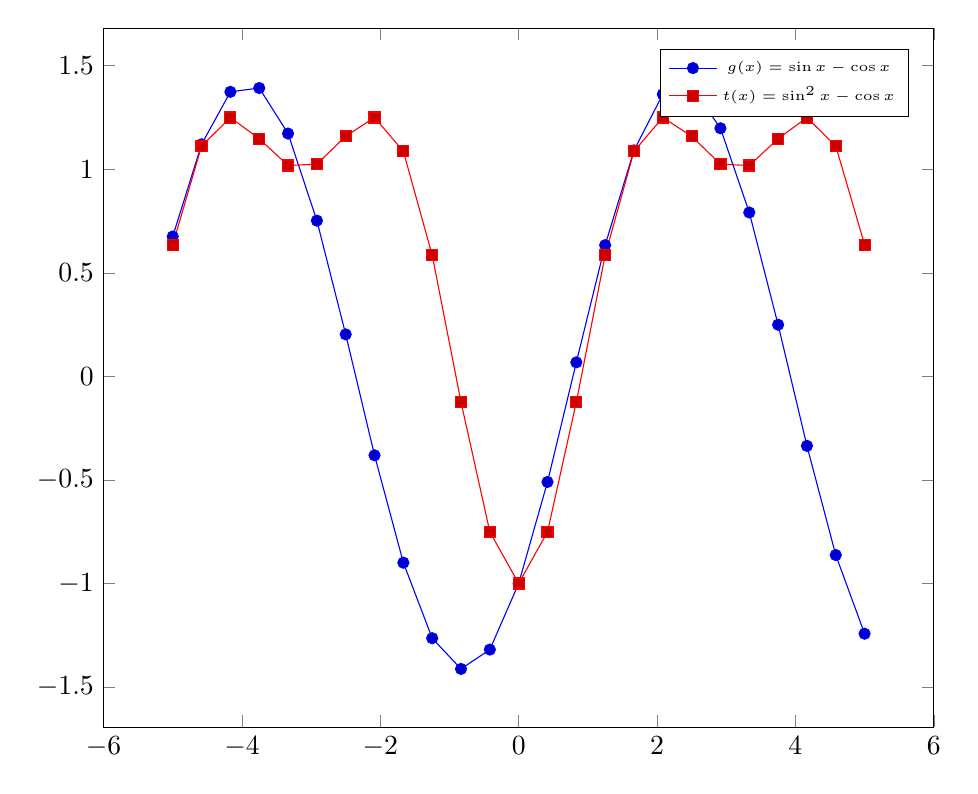
\begin{tikzpicture}
		\begin{axis}[trig format=rad, width=1\linewidth, legend pos=north east, legend style={font=\tiny}]
			\addplot{sin(x) - cos(x)};
			\addlegendentry{$g(x) = \sin x - \cos x$}
			\addplot{sin(x)^2 - cos(x)};
			\addlegendentry{$t(x) = \sin^2 x - \cos x$}
		\end{axis}
	\end{tikzpicture}
	\caption{Plot of $g(x)$ and $t(x)$}
\end{subfigure}
\hfill
\begin{subfigure}{0.32\textwidth}\centering
	\begin{tikzpicture}
		\begin{axis}[width=1\linewidth, legend pos=north east, legend style={font=\tiny}]
			\addplot[variable=\alpha]{e^(\alpha) + \alpha * ln(\alpha)};
			\addlegendentry{$\theta(\alpha) = e^\alpha + \alpha \ln \alpha$}
		\end{axis}
	\end{tikzpicture}
	\caption{Plot of $\theta(\alpha)$}
\end{subfigure}


		\caption{Plots of functions}
		\label{fig:plot}
	\end{figure}
\end{answer}

% \vec{B} + (-\vec{B}) = 0
\begin{answer}[Vector subtraction]
	The rule for vector subtraction is to add the augend add the result of reversing the direction of the addend.

	Any vectors $\vec{A}$ and $\vec{B}$ satisfy the following equation.
	\begin{align}
		\vec{A} - \vec{B} & = \vec{A} + \left(-\vec{B}\right)
	\end{align}
\end{answer}

% calculation
\begin{answer}[Vector magnitude]
	For any vector $\vec{A}$, the magnitude $\left| \vec{A} \right| = \sqrt{A_x^2 + A_y^2 + A_z^2}$ of $\vec{A}$ satisfies the following equations:
	\begin{align}
		\vec{A} \cdot \vec{A} & = A_x A_x + A_y A_y + A_z A_z & = \left| \vec{A} \right|^2.
	\end{align}
\end{answer}

% calculation
\begin{answer}[Magnitudes]
	Let $\left(A_x = 2, A_y = -3, A_z = 1\right)$ and $\left(B_x=-4, B_y=-3, B_z=2\right)$.

	The magnitude $\left|\vec{A}\right| = \sqrt{2^2 + (-3)^2 + 1^2}$ of $\vec{A}$ is $\left|\vec{A}\right| = \sqrt{4+9+1} = \sqrt{14}$, and the magnitude $\left|\vec{B}\right| = \sqrt{(-4)^2 + (-3)^2 + 2^2}$ of $\vec{B}$ is $\left|\vec{B}\right| = \sqrt{29}$.
	The dot product $\vec{A} \cdot \vec{B} = 2(-4) + (-3)(-3) + 1(2)$ of $\vec{A}$ and $\vec{B}$ is $\vec{A} \cdot \vec{B} = 3$.
	Since the angle $\theta$ between the two vectors satisfies $\vec{A} \cdot \vec{B} = \left|\vec{A}\right| \left|\vec{B}\right| \cos \theta$, it is given by $\dsp \theta = \cos^{-1} \frac{3}{\sqrt{406}}$ and approximated by $1.421$ radians.
\end{answer}

% dot product
\begin{answer}[Orthogonality]
	Consider the vectors below.
	\begin{align}
		\left\{(1,1,1), (2,-1,3), (3,1,0), (-3,0,2)\right\}
	\end{align}
	The only pair of orthogonal vectors is $\left\{(2,-1,3), (-3,0,2)\right\}$.
\end{answer}

% orthogonal angle is pi/2
\begin{answer}[Dot product of orthogonal vectors]
	The angle $\theta$ between two vectors that are orthogonal $\vec{A} \perp \vec{B}$ is $\frac{\pi}{2}$ radians, so their dot product is shown below.
	\begin{align}
		\vec{A} \cdot \vec{B} & = \left|\vec{A}\right| \left|\vec{B}\right| \cos \frac{\pi}{2} = 0
	\end{align}
\end{answer}

\subsection{Motion}

% calculation
\begin{answer}[First derivatives]
	Consider the functions $f,g,\theta,t$ defined by $f(t) = t^4 + 3t^3 - 12t^2 + t - 6$, $g(x) = \sin x - \cos x$, $\theta(\alpha) = e^\alpha + \alpha \ln \alpha$, and $t(x) = \sin^2x - \cos x$.

	The derivatives are given below.
	\begin{align*}
		\frac{df}{dt}           & = 4t^3 + 9t^2 - 24t + 1                \\
		\frac{dg}{dx}           & = \cos x + \sin x                      \\
		\frac{d\theta}{d\alpha} & = e^\alpha + 1 + \ln \alpha            \\
		\frac{dt}{dx}           & = \left(2 \sin x\right)\cos x + \sin x
	\end{align*}
\end{answer}

% calculation
\begin{answer}[Second derivatives]
	Consider the functions $f,g,\theta,t$ defined by $f(t) = t^4 + 3t^3 - 12t^2 + t - 6$, $g(x) = \sin x - \cos x$, $\theta(\alpha) = e^\alpha + \alpha \ln \alpha$, and $t(x) = \sin^2x - \cos x$.

	The second derivatives are given below.
	\begin{align*}
		\frac{d^2f(t)}{dt^2}                & = 12t^2 + 18t - 24                                                   \\
		\frac{d^2g(x)}{dx^2}                & = \cos x - \sin x                                                    \\
		\frac{d^2\theta(\alpha)}{d\alpha^2} & = e^\alpha + \frac{1}{\alpha}                                        \\
		\frac{d^2t(x)}{dx^2}                & = -\left(2\sin x\right)\sin x + \left(2 \cos x\right)\cos x + \cos x
	\end{align*}
\end{answer}

% chain rule
\begin{answer}[Chain rule]
	Consider the functions $g,\theta,x$ defined by $g(t) = \sin t^2 - \cos t^2$, $\theta(\alpha) = e^{3 \alpha} + 3 \alpha \ln 3 \alpha$, and $x(t) = \sin^2 t^2 - \cos t^2$.

	The chain rule yields the following derivatives.
	\begin{align*}
		\frac{dg}{dt}           & = 2t \cos t^2 + 2t \sin t^2          \\
		\frac{d\theta}{d\alpha} & = 3e^{3\alpha} + 3 + 3\ln 3\alpha    \\
		\frac{dx}{dt}           & = 4t(\sin t^2)\cos t^2 + 2t \sin t^2
	\end{align*}
\end{answer}

% multiplication by 1
\begin{answer}
	The sum rule is shown for any $f$ and $g$ below.
	\begin{align*}
		\frac{d(f+g)}{dt} & =
		\lim_{\Delta t \to 0} \frac{\left(f(t+\Delta t)+g(t+\Delta t)\right)-\left(f(t)+g(t)\right)}{\Delta t}                                      \\
		                  & = \lim_{\Delta t \to 0} \frac{\left(f(t+\Delta t)-f(t)\right)+\left(g(t+\Delta t)-g(t)\right)}{\Delta t}                \\
		                  & = \lim_{\Delta t \to 0} \frac{f(t+\Delta t)-f(t)}{\Delta t} + \lim_{\Delta t \to 0} \frac{g(t+\Delta t)-g(t)}{\Delta t} \\
		                  & = \frac{df}{dt} + \frac{dg}{dt}
	\end{align*}
	The product rule for any differentiable functions $f$ and $g$ is shown below.
	\begin{align*}
		\frac{d}{dt}\left(f(t) g(t)\right)
		 & = \lim_{\Delta t \to 0} \frac{f(t+\Delta t) g(t+\Delta t) - f(t)g(t)}{\Delta t}                                                                                                                                        \\
		 & = \lim_{\Delta t \to 0} \frac{f(t+\Delta t) g(t+\Delta t) - f(t) g(t) - f(t) g(t+\Delta t) + f(t) g(t+\Delta t)}{\Delta t}                                                                                             \\
		 & = \lim_{\Delta t \to 0} \left(g(t+\Delta t) \frac{f(t+\Delta t) - f(t)}{\Delta t}\right) + \lim_{\Delta t \to 0} f(t) \frac{g(t+\Delta t) - g(t)}{\Delta t}                                                            \\
		 & = \lim_{\Delta t \to 0} \left(g(t+\Delta t) \frac{f(t+\Delta t) - f(t)}{\Delta t}\right) + \lim_{\Delta t \to 0} f(t) \lim_{\Delta t \to 0} \frac{g(t+\Delta t) - g(t)}{\Delta t}                                      \\
		 & = \left(\lim_{\Delta t \to 0} g(t + \Delta t)\right) \left(\lim_{\Delta t \to 0} \frac{f(t+\Delta t) - f(t)}{\Delta t}\right) + \lim_{\Delta t \to 0} f(t) \lim_{\Delta t \to 0} \frac{g(t+\Delta t) - g(t)}{\Delta t} \\
		 & = g(t) \frac{d(f)}{dt} + f(t) \frac{d(g)}{dt}
	\end{align*}
	The chain rule for any $f$ and $g$ is trivial where $g$ is locally constant near $t$, and it is shown below in regions where there is a sufficiently small $\Delta t$ such that $g(t+\Delta t) \neq g(t)$.
	\begin{align*}
		\frac{d\left(f(g(t))\right)}{dt}
		 & = \lim_{\Delta t \to 0} \left[ \frac{f\left(g(t+\Delta t)\right) - f\left(g(t)\right)}{\Delta t} \cdot \frac{g(t + \Delta t) - g(t)}{g(t + \Delta t) - g(t)} \right]                              \\
		 & = \left[\lim_{\Delta t \to 0} \frac{f\left(g(t+\Delta t)\right) - f\left(g(t)\right)}{g(t + \Delta t) - g(t)} \right] \left[\lim_{\Delta t \to 0 }\frac{g(t + \Delta t) - g(t)}{\Delta t} \right] \\
		 & = \left[\frac{d\left(f(g)\right)}{dg}\right]_{g=g(t)} \frac{dg}{dt}
	\end{align*}
\end{answer}

% \theta < \tan \theta
\begin{answer}[Trigonometry]
	Recall the angle addition formula given below.
	\begin{align}
		\sin\left(\alpha + \beta\right) & = \sin \alpha \cos \beta + \cos \alpha \sin \beta \\
		\cos\left(\alpha + \beta\right) & = \cos \alpha \cos \beta - \sin \alpha \sin \beta \\
	\end{align}
	Let $D_+ = \left(0, \frac{\pi}{2}\right)$, $D_- = \left(-\frac{\pi}{2}, 0\right)$, and $D = D_- \cup D_+$.
	Recall that any $\theta \in D_+$ satisfies $\dsp \sin \theta < \theta < \tan \theta$.
	Division by $\theta$ yields $\dsp \frac{\sin \theta}{\theta} < 1 < \frac{\tan \theta}{\theta}$ and multiplication by $\cos \theta$ yields $\cos \theta < \frac{\sin \theta}{\theta}$ since $\cos \theta > 0$ on $D_+$.
	This yields the inequalities $\dsp \cos \theta < \frac{\sin \theta}{\theta} < 1$ on $D_+$.
	If $\theta \in D_-$, then $u = - \theta$ satisfies $\frac{\sin \theta}{\theta} = \frac{\sin -u}{-u} = \frac{\sin u}{u}$ since sine is odd and $\cos\p{-u} = \cos\p{u}$ since cosine is even.
	By symmetry, the same inequality holds on $D_-$ and thus $D$.
	It follows from continuity of sine that $\dsp \lim_{\theta \to 0} \sin \theta = \sin 0 = 0$ and similarly that $\dsp \lim_{\theta \to 0} \cos \theta = \cos 0 = 1$.
	Since $\dsp \cos \theta < \frac{\sin \theta}{\theta} < 1$, the squeeze theorem yields $\dsp \lim_{\theta \to 0} \frac{\sin \theta}{\theta} = 1$.
	Since $\dsp \lim_{\Delta t \to 0} \cos \Delta t = 1$ and $\dsp \lim_{\Delta t \to 0} \p{\cos \Delta t+1} = 2 \neq 0$, it follows that $\dsp \lim_{\Delta t \to 0} \frac{\sin \Delta t}{\cos \Delta t + 1} = \frac{\lim_{\Delta t \to 0} \sin \Delta t}{\lim_{\Delta t \to 0} \left(\cos \Delta t + 1\right)} = \frac{0}{2} = 0$.
	Since it also holds that $\dsp \lim_{\Delta t \to 0} \sin \Delta t = 0$, it also follows that $\dsp \lim_{\Delta t \to 0} \frac{\cos \Delta t - 1}{\Delta t} = \lim_{\Delta t \to 0} \left[- \frac{\sin \Delta t}{\Delta t} \frac{\sin \Delta t}{\cos \Delta t + 1}\right] = 0$.

	Observe $\dsp \frac{d\left(\sin t\right)}{dt} = \lim_{\Delta t \to 0} \frac{\left(\sin t \cos \Delta t + \cos t \sin \Delta t\right) - \sin(t)}{\Delta t} = \lim_{\Delta t \to 0} \left[\frac{\cos \Delta t - 1}{\Delta t} \sin t + \frac{\sin \Delta t}{\Delta t} \cos t\right] = \cos t$ and $\dsp \frac{d\left(\cos t\right)}{dt} = \lim_{\Delta t \to 0} \frac{\left(\cos t \cos \Delta t - \sin t \sin \Delta t\right) - \cos t}{\Delta t} = - \sin t$.

	It follows from the definition of $e^t$ in \cite[p. 34]{TM} that $\dsp \frac{d\left(e^t\right)}{dt} = e^t$.

	If $x = \ln t$ for $t>0$, then the derivative of $t = e^x$ satisfies the equations $\dsp 1 = \frac{dt}{dt} = \frac{d}{dt}\p{e^{x(t)}} = e^{x(t)} \frac{dx}{dt}$ and $\dsp \frac{d}{dt}\p{\ln t} = \frac{dx}{dt} = \frac{1}{e^{x(t)}} = \frac{1}{t}$.
\end{answer}

% 2 \pi = \omega \times period
\begin{answer}[Period]
	If the position of the particle is governed by $x(t) = \sin \omega t$, then the amount of time it takes for the oscillating particle to go through one full cycle of motion is given below.
	\begin{align}
		\frac{2 \pi}{\omega}
	\end{align}
\end{answer}

% calculation
\begin{answer}
	The dot product of the position and velocity vectors is given below.
	\begin{align}
		\vr \cdot \dot{vr}
		 & =
		\begin{bmatrix}
			R \cos \omega t \\
			R \sin \omega t
		\end{bmatrix}
		\cdot
		\begin{bmatrix}
			-R \omega \sin \omega t \\
			R \omega \cos \omega t
		\end{bmatrix} \nonumber \\
		 & =
		- (R \cos \omega t)(R \omega \sin \omega t) + (R \sin \omega t)(R \omega \cos \omega t)
	\end{align}
	Since their dot product is $0$, the vectors are orthogonal.
\end{answer}

% calculation
\begin{answer}
	The position vector $\dsp \vec{r} = \left(\cos \omega t, e^{\omega t}\right)$ has velocity $\left(-\omega \sin \omega t, \omega e^{\omega t}\right)$, acceleration $\left(-\omega^2 \cos \omega t, \omega^2 e^{\omega t}\right)$, and speed $\omega \sqrt{\sin^2 \omega t + e^{2 \omega t}}$.
	The position vector $\dsp \vec{r} = \left(\cos(\omega t - \phi), \sin(\omega t - \phi)\right)$ has velocity $\dsp \left(-\omega \sin(\omega t - \phi), \omega \cos(\omega t - \phi)\right)$, acceleration $\dsp \left(-\omega^2 \cos(\omega t-\phi), -\omega^2\sin(\omega t-\phi)\right)$, and speed $\omega$.
	The position vector $\dsp \left(c \cos^3 t, c \sin^3 t\right)$ has velocity $\dsp \left(-3c (\sin t)\cos^2 t, 3c(\cos t)\sin^2 t\right)$, acceleration $\dsp \left(6c (\cos t)\sin^2 t - 3c\cos^3 t, 6c (\sin t)\cos^2 t - 3c\sin^3 t\right)$, and speed $3\left| c (\sin t)(\cos t) \right|$.
	The position vector $\dsp \vec{r} = \left(c(t-\sin t), c(1-\cos t)\right)$ has velocity $\dsp \left(c - c\cos t, c\sin t\right)$, acceleration $\dsp \left(c\sin t,  c\cos t\right)$, and speed $\dsp c\sqrt{2(1- \cos t)}$.
\end{answer}

\subsubsection{Integral calculus}
\setcounter{answer}{0}

% linearity
\begin{answer}
	Consider the functions $f_1, f_2, f_3$ defined below.
	\begin{align}
		f_1(t) & = t^4     \\
		f_2(t) & = \cos t  \\
		f_3(t) & = t^2 - 2
	\end{align}
	The indefinite integrals of $f_1$ and $f_2$ are $\dsp \int t^4 ~dt = \frac{t^5}{5} + c$ and $\dsp \int \cos t ~dt = \sin t + c$.
	Finally, linearity of the integral yields $\dsp \int (t^2 - 2) dt = \frac{t^3}{3} - 2t + c$.
\end{answer}

% direct integration
\begin{answer}
	The fundamental theorem of calculus yields $\dsp \int_0^T t^4 ~dt = \frac{T^5}{5} - \frac{0^5}{5}$, $\dsp \int_0^T \cos t ~dt= \sin T - \sin 0$, and $\dsp \int_0^T \p{t^2-2} dt = \frac{T^3}{3} - 2T$.
\end{answer}

% direct integration
\begin{answer}
	The velocities $\dsp v_1(t) = \int_0^t {t'}^4~dt'$, $\dsp v_2(t) = \int_0^t \cos t' ~dt'$, $\dsp v_3(t) = \int_0^t \left({t'}^2-2\right) ~dt'$ has trajectories $\dsp \int_0^T \left(\frac{t^5}{5} - \frac{0}{5}\right) ~dt = \frac{T^6}{30} - 0$, $\dsp \int_0^T \sin t - 0 ~dt = - \cos T + 1$, and $\dsp \int_0^T \frac{t^3}{3}-2t ~dt = \frac{T^4}{12}-T^2$.
\end{answer}

% parts
\begin{answer}
	Calculating $\dsp \int_0^{\frac{\pi}{2}} x \cos x ~dx = \frac{\pi}{2}\sin \frac{\pi}{2} - \int_0^{\frac{\pi}{2}} \sin x ~dx$ yields the following integral.
	\begin{align}
		\int_0^{\frac{\pi}{2}} \left(x \cos x\right) dx = \frac{\pi}{2} \sin \frac{\pi}{2} - 1
	\end{align}
\end{answer}

\subsection{Dynamics}

% power
\begin{answer}
	If a force varies with time according to $F = 2t^2$ and with initial condition $x(0) = \pi$ at time $0$, then Aristotle's law of motion $\dsp \int \frac{dx(t)}{dt}~dt = \int \frac{F(t)}{m}~dt$ yields $\dsp x(t) = \frac{2t^3}{3m} + c$ where $\dsp \pi = \frac{2\cdot 0^3}{3m} + c$ implies $c = \pi$.
\end{answer}

% fundamental theorem of calculus
\begin{answer}
	For a constant force $F_z$, integrating $\dsp \int_0^t \dot{v_z} = \int_0^t \frac{F_z}{m}$ yields the following equation.
	\begin{align}
		v_z(t) & = v_z(0) + \frac{F_z}{m}t
	\end{align}
\end{answer}

% power
\begin{answer}
	Consider a constant force on a body with a constant mass $m$.

	Differentiating $\dsp z(t) = z_0 + v_z(0)t + \frac{F_z}{2m}t^2$ yields the following velocity.
	\begin{align}\label{eqn:vel}
		v_z(t) & = v_z(0) + \frac{F_z}{m}t
	\end{align}
	Differentiating Equation \eqref{eqn:vel} yields $\dsp \dot{v_z}(t) = \frac{F_z}{m}$.
	This is the equation of motion for a constant force on a body with constant mass.
\end{answer}

% chain rule
\begin{answer}
	The derivative of $\dsp x(t) = A \cos\p{\omega t} + B \sin\p{\omega t}$ is given below.
	\begin{align}
		\dot{x}(t) & = -\omega A \sin\p{\omega t} + \omega B \cos\p{\omega t}
	\end{align}
	The second derivative is $\ddot{x}(t) = -\omega^2 A \cos\p{\omega t} - \omega^2 B \sin\p{\omega t} = -\omega^2 x(t)$.
	The initial position at time $t=0$ is $x(0) = A$, and the initial velocity at time $t=0$ is $B\omega$.
\end{answer}

\subsubsection{Partial differentiation}
\setcounter{answer}{0}

% calculation
\begin{answer}
	Consider the functions $V_1,V_2,V_3$ defined below.
	\begin{align}
		V_1(x,y) & = x^2 + y^2 - \sin\p{x y} \\
		V_2(x,y) & = \frac{x}{y} e^{x^2+y^2} \\
		V_3(x,y) & = e^x \cos y
	\end{align}
	The first derivatives are calculated below.
	\begin{align*}
		\frac{\partial V_1}{\partial x} & = 2x - y \cos xy
		                                & \frac{\partial V_1}{\partial y}                        & = 2y - x \cos xy                                                                \\
		\frac{\partial V_2}{\partial x} & = \left(\frac{2x^2}{y} + \frac{1}{y}\right)e^{x^2+y^2} & \frac{\partial V_2}{\partial y} & = \left(2x - \frac{x}{y^2} \right)e^{x^2+y^2} \\
		\frac{\partial V_3}{\partial x} & = e^x \cos y                                           & \frac{\partial V_3}{\partial y} & = -e^x \sin y
	\end{align*}
	The second derivatives are given below.
	\begin{align*}
		\frac{\partial^2 V_1}{\partial x^2} & = 2 + y^2 \sin xy
		                                    & \frac{\partial^2 V_1}{\partial y^2}                     & = 2 + x^2\sin xy
		                                    & \frac{\partial^2 V_1}{\partial x \partial y}            & = - \cos\p{x y} + xy \sin\p{x y}                                                                                                                                     \\
		\frac{\partial^2 V_2}{\partial x^2} & = \left(\frac{4x^3}{y} + \frac{6x}{y}\right)e^{x^2+y^2}
		                                    & \frac{\partial^2 V_2}{\partial y^2}                     & = \left(4xy - \frac{2x}{y} + \frac{2x}{y^3}\right)e^{x^2+y^2} & \frac{\partial^2 V_2}{\partial x \partial y} & = \left(4x^2+2 - \frac{1+2x^2}{y^2}\right)e^{x^2+y^2} \\
		\frac{\partial^2 V_3}{\partial x^2} & = e^x \cos y
		                                    & \frac{\partial^2 V_3}{\partial y^2}                     & = - e^x \cos y
		                                    & \frac{\partial^2 V_3}{\partial x \partial y}            & = -e^x \sin y
	\end{align*}
\end{answer}

% test of second derivative
\begin{answer}
	The functions $F_1(x,y) = \sin x + \sin y$ and $F_2(x,y) = \cos x + \cos y$ have the first derivatives below.
	\begin{align*}
		\frac{\partial F_1}{\partial x} & = \cos x  & \frac{\partial F_1}{\partial y} & = \cos y  \\
		\frac{\partial F_2}{\partial x} & = -\sin x & \frac{\partial F_2}{\partial y} & = -\sin y
	\end{align*}

	The Hessians are calculated below.
	\begin{align*}
		H_1(x,y) & =
		\begin{pmatrix}
			\frac{\partial^2 F_1}{\partial x^2}          & \frac{\partial^2 F_1}{\partial x \partial y} \\
			\frac{\partial^2 F_1}{\partial y \partial x} & \frac{\partial^2 F_1}{\partial y^2}
		\end{pmatrix}
		=
		\begin{pmatrix}
			- \sin x & 0       \\
			0        & -\sin y
		\end{pmatrix}
		\\
		H_2(x,y) & =
		\begin{pmatrix}
			\frac{\partial^2 F_2}{\partial x^2}          & \frac{\partial^2 F_2}{\partial x \partial y} \\
			\frac{\partial^2 F_2}{\partial y \partial x} & \frac{\partial^2 F_2}{\partial y^2}
		\end{pmatrix}
		=
		\begin{pmatrix}
			- \cos x & 0        \\
			0        & - \cos y
		\end{pmatrix}
	\end{align*}

	The determinants are given below.
	\begin{align*}
		\op{Det} H_1 & = \frac{\partial^2 F_1}{\partial x^2} \frac{\partial^2 F_1}{\partial y^2} - \frac{\partial^2 F_1}{\partial y \partial x}\frac{\partial^2 F_1}{\partial x \partial y} = \sin x \sin y - 0 \\
		\op{Det} H_2 & = \frac{\partial^2 F_2}{\partial x^2} \frac{\partial^2 F_2}{\partial y^2} - \frac{\partial^2 F_2}{\partial y \partial x}\frac{\partial^2 F_2}{\partial x \partial y} = \cos x \cos y - 0
	\end{align*}

	The point $\dsp \left(\frac{\pi}{2}, -\frac{\pi}{2}\right)$ is a saddle point of $F_1$ and it is not a stationary point of $F_2$.
	The point $\dsp \left(-\frac{\pi}{2}, \frac{\pi}{2}\right)$ is a saddle point of $F_1$ and it is not a stationary point of $F_2$.

	The point $\dsp p = \left(-\frac{\pi}{2}, -\frac{\pi}{2}\right)$ is not a stationary point of $F_2$ since the gradient of $F_2$ does not vanish there.

	The trace of $H_1$ is calculated below.
	\begin{align}
		\op{Tr} H_1 & = \frac{\partial^2 F_1}{\partial x^2} + \frac{\partial^2 F_1}{\partial y^2} = - \sin x - \sin y
	\end{align}
	The point $p$ is a stationary point of $F_1$ since $\nabla F_1(p) = \p{0, 0}$, and it is a local minimum of $F_1$ since $\det H_1\p{p}$ is positive and $\left[\Tr H_1\right]_p$ is positive.
\end{answer}

\subsection{Systems of more than one particle}

There are no exercises in this lecture.

\subsection{Energy}

% product rule
\begin{answer}
	For a particle with a velocity $v(t)$ in one direction, the derivative of $v^2(t) = v(t)^2$ is calculated by the product rule below.
	\begin{align}
		\frac{dv^2}{dt} & = v \dot{v} + \dot{v} v
	\end{align}
	Therefore, the derivative is $\frac{dv^2}{dt} = 2 v \dot{v}$.
\end{answer}

\begin{answer}
	Consider a particle with mass $m$ in two dimensions, $x$ and $y$, in which the potential energy is $V = \frac{1}{2} k \left(x^2+y^2\right)$ and the initial data is given.
	\begin{align*}
		\vr_0
		 & =
		\begin{pmatrix}
			x(0) \\
			y(0)
		\end{pmatrix}
		=
		\begin{pmatrix}
			x_0 \\
			y_0
		\end{pmatrix}
		 &
		\dot{\vr}_0 =
		\begin{pmatrix}
			\dot{x}(0) \\
			\dot{y}(0)
		\end{pmatrix}
		=
		\begin{pmatrix}
			\dot{x}_0 \\
			\dot{y}_0
		\end{pmatrix}
	\end{align*}

	Observe $\dsp \nabla V = \begin{pmatrix} \frac{\partial V}{\partial x} \\ \frac{\partial V}{\partial y} \end{pmatrix} = \begin{pmatrix} kx \\ ky \end{pmatrix}$, and the force $\dsp F = \begin{pmatrix} F_x \\ F_y \end{pmatrix}$ has components $F_x = -kx$ and $F_y = -ky$.
	The equations of motion are $m \ddot{x} = -kx$ and $m \ddot{y} = -ky$.
	The solution is given in terms of $\dsp \omega = \sqrt{\frac{k}{m}}$ below.
	\begin{align}
		\vr
		 & =
		\begin{pmatrix}
			x \\
			y
		\end{pmatrix}
		= \phantom{-\omega^2}
		\begin{pmatrix}
			x_0 \cos \omega t + \frac{\dot{x}_0}{\omega} \sin \omega t \\
			y_0 \cos \omega t + \frac{\dot{y}_0}{\omega} \sin \omega t
		\end{pmatrix}  \\
		\dot{\vr}
		 & =
		\begin{pmatrix}
			\dot{x} \\
			\dot{y}
		\end{pmatrix}
		=
		\phantom{-} \omega
		\begin{pmatrix}
			-x_0 \sin \omega t + \frac{\dot{x}_0}{\omega} \cos \omega t \\
			-y_0 \sin \omega t + \frac{\dot{y}_0}{\omega} \cos \omega t
		\end{pmatrix} \nonumber \\
		\ddot{\vr}
		 & =
		\begin{pmatrix}
			\ddot{x} \\
			\ddot{y}
		\end{pmatrix}
		=
		- \omega^2
		\begin{pmatrix}
			x_0 \cos \omega t +  \frac{\dot{x}_0}{\omega} \sin \omega t \\
			y_0 \cos \omega t + \frac{\dot{y}_0}{\omega} \sin \omega t
		\end{pmatrix}
		= - \frac{k}{m} \vr \nonumber
	\end{align}
	Observe it satisfies the equations and that the orbits have period $\dsp 2\pi \sqrt{\frac{m}{k}}$.

	Let $\dsp \vb = \frac{\vr_0}{\omega}$.
	The orbit is an ellipse centered at the origin whose principal axes are along the eigenvectors of the matrix $\vr_0 \vr_0^\top + \mbf{b} \mbf{b}^\top$.
	It is a circle if $\left|\dot{\vr}_0\right| = \omega \left|\vr_0\right|$ and $\vr_0 \cdot \dot{\vr}_0 = 0$.

	Since $\dsp V = \frac{k}{2} \left|\vr\right|^2$, it follows from the chain rule that $\dot{V} = k \vr \cdot \dot{\vr}$ and from the equation of motion that $\dsp \dot{T} = m \dot{\vr} \cdot \ddot{\vr} = - k \vr \cdot \dot{\vr}$.
	Addition yields $\dsp \dot{E} = \dot{T} + \dot{V} = 0$.
	Thus, the total energy is conserved.
\end{answer}

\begin{answer}
	Consider a particle with mass $m$ in two dimensions, $x$ and $y$, with potential energy $\dsp V = \frac{k}{2(x^2+y^2)}$.

	Let $\vr = \begin{pmatrix} x \\ y \end{pmatrix} = \begin{pmatrix} r \cos \theta \\ r \sin \theta \end{pmatrix}$, $r = \left|\vr\right|$, $\dsp \widehat{\vr} = \frac{\vr}{r}$, and $\dsp V' = \frac{dV}{dr} = \frac{d}{dr}\left(\frac{k}{2r^2}\right) = \frac{-k}{r^{3}}$.

	The chain rule yields the gradient below.
	\begin{align*}
		\nabla V & = \begin{pmatrix} \frac{\partial V}{\partial x} \\ \frac{\partial V}{\partial y}\end{pmatrix}
		=
		k
		\begin{pmatrix}
			-\frac{x}{(x^2+y^2)^2} \\
			-\frac{y}{(x^2+y^2)^2}
		\end{pmatrix}
		= -\frac{k}{r^4} \vr
		         &
		F        & = -\nabla V = k
		\begin{pmatrix}
			\frac{x}{(x^2+y^2)^2} \\
			\frac{y}{(x^2+y^2)^2}
		\end{pmatrix}
		= \frac{k}{r^4}\vr
		= - V'(r) \widehat{\vr}
	\end{align*}
	The equations of motion are $\dsp m \ddot{x} = k\frac{x}{(x^2+y^2)^2}$ and $\dsp m \ddot{y} = k \frac{y}{(x^2+y^2)^2}$.
	Let $\dsp \widehat{\vth} = \begin{pmatrix} - \sin \theta \\ \cos \theta \end{pmatrix}$.
	Differentiation yields $\dot{\widehat{\vr}} = \dot{\theta} \widehat{\vth}$, $\dot{\widehat{\vth}} = - \dot{\theta} \widehat{\vr}$, $\dot{\vr} = r \dot{\theta} \widehat{\vth} + \dot{r} \widehat{\vr}$, and $\ddot{\vr} = \left(\ddot{r} - r \dot{\theta}^2\right) \widehat{\vr} + \left(r \ddot{\theta} + 2 \dot{r} \dot{\theta}\right) \widehat{\vth}$.
	The equivalent equations of motion are $m\left(\ddot{r} - r\dot{\theta}^2\right) = F_r = \frac{k}{r^3}$ and $m\left(r\ddot{\theta} + 2\dot{r}\dot{\theta}\right) = F_\theta = 0$.

	Let $\dsp L = mr^2 \dot{\theta}$, $\dsp T = \frac{m}{2}\left(\dot{\vr} \cdot \dot{\vr}\right)$, $\dsp u(\theta) = \frac{1}{r(\theta)}$, $\dsp r' = \frac{dr}{d\theta}$, and $\dsp r'' = \frac{d^2r}{d\theta^2}$.
	Note $\dsp \dot{L} = mr^2\ddot{\theta} + 2mr\dot{r} \dot{\theta} = r F_\theta = 0$ and $\dsp \dot{\theta} = \frac{L}{mr^2}$.
	Substitution yields $\dsp F_r = m\ddot{r} - \frac{L^2}{mr^3}$.
	Observe that $\dsp u' = \frac{du}{d\theta} = \frac{-r'}{r^2}$ and $\dsp u'' = \frac{d^2u}{d\theta^2}$.
	Then, $\dot{r} = -\frac{L}{m} u'$ and $\ddot{r} = - \frac{L^2}{m^2} u^2 u''$.
	Since $\dsp F\!\left(\frac{1}{u}\right) = ku^3$, this yields $\dsp u'' + \alpha^2 u = 0$ where $\dsp \alpha = \sqrt{1 + \frac{mk}{L^2}}$.
	The solution is given by $u(\theta) = A \cos\!\left(\alpha(\theta-\theta_0)\right)$ in terms of the initial data, and thus $\dsp r(\theta) = \frac{1}{A \cos\!\left(\alpha(\theta - \theta_0)\right)}$.

	Let $E = T + V$.
	Recall $\dsp \dot{T} = m \dot{\vr} \cdot \ddot{\vr}$ and observe that $\dsp \dot{E} = \dot{T} + \dot{V} = \dot{T} + \nabla V \cdot \dot{\vr} = \dot{\vr} \cdot \left(m\ddot{\vr} + \nabla V\right) = \dot{\vr} \cdot 0 = 0$.
	Thus, total energy is conserved.

	Assuming $r(t) = R$ for some constant $R$ and all $t$ yields $\dsp -mR \dot{\theta}^2 = \frac{k}{R^3}$ and $\dsp \dot{\theta}^2 = - \frac{k}{mR^4}$.
	There are no elliptic orbits if $k \geq 0$.
	If $k = -\frac{L^2}{m} = - m R^4 \dot{\theta}^2$ for some constant $R$, then the orbit is circular with a period $\frac{2 \pi}{\dot{\theta}} = 2 \pi R^2\sqrt{\frac{m}{-k}}$ that depends on the radius $R$ of the circle.
\end{answer}

\subsection{Principle of least action}

\begin{answer}
	A particle with position $x$ in one dimension has kinetic energy $\dsp T = \frac{m}{2}\left(\dot{x} \cdot \dot{x}\right)$, potential energy $V$, force $\dsp F = - \nabla_x V$, Lagrangian $L = T - V$, and acceleration $a = \ddot{x}$.
	Observe the equations below.
	\begin{align}
		\frac{d}{dt} \frac{\partial L}{\partial \dot{x}} - \frac{\partial L}{\partial x} = \frac{d}{dt} \frac{\partial}{\partial \dot{x}}\!\left(\frac{m}{2} \dot{x} \cdot \dot{x}\right) + \frac{\partial V}{\partial x}
		= \frac{d}{dt}\!\left(m \dot{x}\right) - F
		= m \ddot{x} - F
	\end{align}
	Therefore, the Euler-Lagrange equation $\frac{d}{dt} \frac{\partial L}{\partial \dot{x}} - \frac{\partial L}{\partial x}=0$ is equivalent to $F = ma$.
\end{answer}

\begin{answer}
	Let $X = \left\{x_i\right\}_{i=1}^N$ be coordinates, $\dsp T = \sum_{i=1}^N \frac{m_i}{2} \dot{x_i}^2$ be the kinetic energy, $V$ be the potential energy, $L = T - V$, and $\dsp F_i = - \frac{\partial V}{\partial x_i}$ for each $i$.

	For any $i$, observe the equations below.
	\begin{align}
		\frac{d}{dt}\!\left(\frac{\partial L}{\partial \dot{x_i}}\right) - \frac{\partial L}{\partial x_i}
		 & = \frac{d}{dt} \frac{\partial}{\partial \dot{x_i}}\!\left(\sum_{j=1}^N \frac{m_j}{2} \dot{x_j}^2\right) + \frac{\partial V}{\partial x_i}
		= \frac{d}{dt}\!\left(m_i\dot{x_i}\right) - F_i = m_i\ddot{x_i} - F_i
	\end{align}
	For any $i$, the Euler-Lagrange equation $\dsp \frac{d}{dt}\!\left(\frac{\partial L}{\partial \dot{x_i}}\right) = \frac{\partial L}{\partial x_i}$ is therefore equivalent to $F_i = m_i \ddot{x_i}$.
\end{answer}

\begin{answer}
	The position of a particle is given in George's coordinate frame by $X$ and $Y$.
	Lenny's coordinate frame is rotating relative George's frame at an angular velocity $\omega$, and the particle is given in Lenny's coordinate frame by $x = X \cos \omega t + Y \sin \omega t$ and $y = -X \sin \omega t + Y \cos \omega t$.
	Suppose the Lagrangian is given in Lenny's coordinate frame by $\dsp L = \frac{m}{2}\left(\dot{x}^2 + \dot{y}^2\right)$.
	If the kinetic energy is $T = \frac{m}{2}\left(\dot{X}^2 + \dot{Y}^2\right)$ and the (velocity-dependent) effective potential energy is $V = -\frac{m \omega^2}{2}\left(X^2 + Y^2\right) - m \omega \left(\dot{X} Y - \dot{Y} X\right)$, then the Lagrangian is given in George's coordinate frame by the expansion of $L = T - V$ in Equation \eqref{eqn:L} below.
	\begin{align}\label{eqn:L}
		L & =  \frac{m}{2}\left(\dot{X}^2 + \dot{Y}^2\right) - \left(-\frac{m \omega^2}{2}(X^2 + Y^2) - m \omega (\dot{X} Y - \dot{Y} X) \right)
	\end{align}
	The Euler-Lagrange equations are $\dsp \frac{d}{dt}\!\left(\frac{\partial L}{\partial \dot{X}}\right) = \frac{\partial L}{\partial X}$ and $\dsp \frac{d}{dt}\!\left(\frac{\partial L}{\partial \dot{Y}}\right) = \frac{\partial L}{\partial Y}$.
	To derive the equations of motion from the Lagrangian $L$, observe $\dsp \frac{\partial L}{\partial X} = - \frac{\partial V}{\partial X} = m\omega^2 X - m \omega \dot{Y}$ and $\dsp \frac{\partial L}{\partial Y} = - \frac{\partial V}{\partial Y} = m \omega^2 Y + m \omega \dot{X}$.
	Since $\dsp \frac{\partial L}{\partial \dot{X}} = m \dot{X} + m \omega Y$ and $\dsp \frac{\partial L}{\partial \dot{Y}} = m \dot{Y} - m \omega X$, it follows that $\dsp \frac{d}{dt}\!\left(\frac{\partial L}{\partial \dot{X}}\right) = m\ddot{X} + m \omega \dot{Y}$ and $\dsp \frac{d}{dt}\!\left(\frac{\partial L}{\partial \dot{Y}}\right) = m \ddot{Y} - m \omega \dot{X}$.
	The equations of motion are given in George's coordinate frame by $m\ddot{X} = m \omega^2 X - 2 m \omega \dot{Y}$ and $m \ddot{Y} = m \omega^2 Y + 2 m \omega \dot{X}$.
\end{answer}

\begin{answer}
	The position of a particle is given in George's frame by polar coordinates $X = R \cos \theta$ and $Y = R \sin \theta$.
	Its velocity is given in polar coordinates by $\dot{X} = \dot{R} \cos \theta - R \dot{\theta} \sin \theta$ and $\dot{Y} = \dot{R} \sin \theta + R \dot{\theta} \cos \theta$.
	Substitution into Equation \eqref{eqn:L} yields George's Lagrangian below.
	\begin{align}\label{eqn:polarL}
		L & =  \frac{m}{2}\left(\dot{R}^2 + R^2 \dot{\theta}^2\right) - \left(-\frac{m \omega^2}{2} R^2 + m \omega R^2 \dot{\theta}\right)
	\end{align}
	The equations of motion are then given by $m \ddot{R} = m R \dot{\theta}^2 + m \omega^2 R - 2 m \omega R \dot{\theta}$ and $2 m R \dot{R} \dot{\theta} + m R^2 \ddot{\theta} - 2 m \omega R \dot{R} = 0$.
\end{answer}

\begin{answer}[Pendulum]\label{ans:pendulum}
	The position $\begin{pmatrix} r \\ \theta \end{pmatrix}$ of a pendulum with length $l$ and mass $m$ must satisfy the equations $r=l$ and $\dot{r} = 0$.
	This allows the use of a single generalized coordinate $\theta$.
	Pick it so that the potential energy at $\theta=0$ is zero.
	Its kinetic energy is given by $T = \frac{m}{2} l^2 \dot{\theta}^2$.
	The height of the pendulum mass is given by $h = l - l \cos \theta$, and its potential energy by $V = mgl\left(1 - \cos \theta\right)$.
	Thus, its Lagrangian by $L = T - V$ is given below.
	\begin{align}\label{eqn:Lpend}
		L & = \frac{m}{2} l^2 \dot{\theta}^2 - mgl\left(1 - \cos \theta\right)
	\end{align}
	Therefore, the angular equation of motion is given by $m l^2 \ddot{\theta} + m g l \sin \theta = 0$.
\end{answer}

\begin{answer}
	The temporal derivatives of $x_+ = \frac{x_1 + x_2}{2}$ and $x_- = \frac{x_1 - x_2}{2}$ are $\dot{x_+} = \frac{\dot{x_1} + \dot{x_2}}{2}$ and $\dot{x_-} = \frac{\dot{x_1} - \dot{x_2}}{2}$.
	Expanding $T = m\left(\dot{x_+}^2 + \dot{x_-}^2\right)$ yields $T = m \left(\frac{\dot{x_1}^2 + 2\dot{x_1}\dot{x_2} + \dot{x_2}^2}{2^2} + \frac{\dot{x_1}^2 - 2\dot{x_1}\dot{x_2} + \dot{x_2}^2}{2^2}\right) = \frac{m}{2}\left(\dot{x_1}^2 + \dot{x_2}^2\right)$, which is the kinetic energy.
\end{answer}

\subsection{Symmetries and conservation laws}

\begin{answer}
	Consider the Lagrangian given by Equation \eqref{eqn:Ldiff} below.
	\begin{align}\label{eqn:Ldiff}
		L = \frac{1}{2}\left(\dot{q_1}^2 + \dot{q_2}^2\right) - V\p{q_1 - q_2}
	\end{align}
	The first Euler-Lagrange equation is given by $\dot{p_1} = -V'(q_1-q_2) \cdot \frac{\partial}{\partial q_1}\p{q_1-q_2} = - V'(q_1-q_2)$ and the second Euler-Lagrange equation is given by $\dot{p_2} = - V'(q_1-q_2) \cdot \frac{\partial}{\partial q_2}\p{q_1-q_2} = + V'(q_1-q_2)$.
	The sign difference is due via the chain rule to the sign difference in the argument $q_1-q_2$ of $V$ in $L$.
\end{answer}

\begin{answer}
	Fix constants $a$ and $b$.
	The sum of $b \dot{p_1} = -ab V'\p{a q_1 - b q_2}$ and $a \dot{p_2} = +ab V'\p{a q_1 - b q_2}$ is $b \dot{p_1} + a \dot{p_2} = 0$.
	Since $a$ and $b$ are constant, it follows that $b \dot{p_1} + a \dot{p_2} = \frac{d}{dt}\p{b p_1 + a p_2}$.
	Therefore, the quantity $b p_1 + a p_2$ is conserved.
\end{answer}

\begin{answer}
	Consider any constants $a$, $b$, and $\delta$.

	Observe $a\left(q_1 + b\delta\right) + b\left(q_2 - a \delta\right) = a q_1 + b q_2$.
	Then, any potential of the form $V\p{a q_1 + b q_2}$ is invariant under the transformations $q_1 \to q_1 + b \delta$ and $q_2 \to q_2 - a \delta$.
	The derivatives of $q_1$ and $q_2$ are invariant since the transformations are independent of time.
	Thus, the kinetic energy and the Lagrangian are also invariant under the transformations of $q_1$ and $q_2$.
\end{answer}

\begin{answer}
	Consider the Lagrangian defined below.
	\begin{align}
		L & = \frac{m}{2}\p{(\dot{x} + \dot{y} \delta)^2 + (\dot{y} - \dot{x} \delta)^2} - V\p{(x + y \delta)^2 + (y - x \delta)^2}
	\end{align}
	It satisfies $L = \frac{m}{2}\p{\dot{x}^2 + \dot{y}^2 + (\dot{y}^2 + \dot{x}^2)\delta^2} - V\p{x^2 + y^2 + (y^2 + x^2) \delta^2}$.
	Therefore, the Lagrangian does not change to first order in $\delta$.
\end{answer}

\begin{answer}
	To determine the equation of motion for a simple pendulum of length $l$ and mass $m$ swinging through an arc in the $x,y$ plane from an initial angle of $\theta_0$, recall the Lagrangian given in Equation \eqref{eqn:Lpend}.
	With the constraint $r=l$, the only generalized coordinate is $\theta$ and the Lagrangian depends explicitly on $\theta$.
	Thus, the generalized coordinate $\theta$ is not cyclic and its conjugate momentum is not conserved.
	Dividing the equation of motion obtained in Exercise \ref{ans:pendulum} by the non-zero mass yields $l^2 \ddot{\theta} + g l \sin \theta = 0$.
\end{answer}

\begin{answer}
	Consider a double pendulum with unit masses $m_1 = m_2 = 1$ and unit lengths $l_1 = l_2 = 1$.
	Let $\theta$ denote the angle of the first rod relative to vertical and $\alpha$ denote the angle of the second rod relative to the first rod.
	The first bob has kinetic energy $T_1 = \frac{\dot{\theta}^2}{2}$, and the second bob has kinetic energy $T_2 = \frac{\dot{\theta}^2 + \p{\dot{\theta} + \dot{\alpha}}^2}{2} + \dot{\theta} \left(\dot{\theta} + \dot{\alpha}\right) \cos \alpha$.
	In the absence of gravity, the potential energy is $V = 0$ and the Lagrangian $L = T_1 + T_2 - V$.
	The conjugate momenta are $p_\theta = 3 \dot{\theta} + \dot{\alpha} + \p{2 \dot{\theta} + \dot{\alpha}} \cos \alpha$ and $p_\alpha = \dot{\theta} + \dot{\alpha} + \dot{\theta} \cos \alpha$.
	Their temporal derivatives are given below.
	\begin{align}
		\dot{p_\theta} & = 3 \ddot{\theta} + \ddot{\alpha} + \p{2 \ddot{\theta} + \ddot{\alpha}} \cos \alpha - \dot{\alpha} \p{2 \dot{\theta} + \dot{\alpha}} \sin \alpha \label{eqn:ptheta} \\
		\dot{p_\alpha} & = \ddot{\theta} + \ddot{\alpha} + \ddot{\theta} \cos \alpha - \dot{\theta} \dot{\alpha} \sin \alpha \label{eqn:palpha}
	\end{align}
	Since the potential energy is $V=0$ in the absence of gravity, the Euler-Lagrange equations are $\dot{p_\theta} = 0$ and $\dot{p_\alpha} = -\dot{\theta}\p{\dot{\theta} + \dot{\alpha}} \sin \alpha$.
\end{answer}

\begin{answer}
	The (generalized) angular momentum for the double pendulum in the absence of gravity is given in terms of the conjugate momenta in Equations \eqref{eqn:ptheta}--\eqref{eqn:palpha} by $\dot{p_\theta} = 0$.
	When there is no gravitational field, the angular momentum $p_\theta$ of the first rod is thus conserved.
\end{answer}

